
\documentclass{beamer}

%%%%%%%%%%%%%%%%%%%%%%%%%%%%%%%%%%%%%%%%%%%%%%%%%%%%%%%%%%%%%%%%%%%%%%
% Codificação
%%%%%%%%%%%%%%%%%%%%%%%%%%%%%%%%%%%%%%%%%%%%%%%%%%%%%%%%%%%%%%%%%%%%%%

\usepackage[brazilian]{babel}
\usepackage[utf8]{inputenc}
\usepackage{lmodern}
\usepackage{mathbbol}
\usepackage{multicol}
\usepackage{algorithmic}
\usepackage{tikz}


% Declaracoes em Português
\renewcommand\algorithmicend{\textbf{fim}}
\renewcommand\algorithmicdo{\textbf{faça}}
\renewcommand\algorithmicwhile{\textbf{enquanto}}
\renewcommand\algorithmicfor{\textbf{para}}
\renewcommand\algorithmicif{\textbf{se}}
\renewcommand\algorithmicthen{\textbf{então}}
\renewcommand\algorithmicelse{\textbf{senão}}
\renewcommand\algorithmicreturn{\textbf{retorne}}
\renewcommand\algorithmicrequire{\textbf{Entrada:}}
\renewcommand\algorithmicensure{\textbf{Variáveis:}}

%%%%%%%%%%%%%%%%%%%%%%%%%%%%%%%%%%%%%%%%%%%%%%%%%%%%%%%%%%%%%%%%%%%%%%
% Tema do beamer
%%%%%%%%%%%%%%%%%%%%%%%%%%%%%%%%%%%%%%%%%%%%%%%%%%%%%%%%%%%%%%%%%%%%%%

\usetheme{Warsaw}

\defbeamertemplate*{footline}{shadow theme}{%
\leavevmode%
\hbox{\begin{beamercolorbox}[wd=.5\paperwidth,ht=2.5ex,dp=1.125ex,leftskip=.3cm plus1fil,rightskip=.3cm]{author in head/foot}%
    \usebeamerfont{author in head/foot}\hfill\insertshortauthor
\end{beamercolorbox}%
\begin{beamercolorbox}[wd=.4\paperwidth,ht=2.5ex,dp=1.125ex,leftskip=.3cm,rightskip=.3cm plus1fil]{title in head/foot}%
    \usebeamerfont{title in head/foot}\insertshorttitle\hfill%
\end{beamercolorbox}%
\begin{beamercolorbox}[wd=.1\paperwidth,ht=2.5ex,dp=1.125ex,leftskip=.3cm,rightskip=.3cm plus1fil]{mycolor}%
\hfill\insertframenumber\,/\,\inserttotalframenumber
\end{beamercolorbox}}%
\vskip0pt%
}

%%%%%%%%%%%%%%%%%%%%%%%%%%%%%%%%%%%%%%%%%%%%%%%%%%%%%%%%%%%%%%%%%%%%%%
% Informações da apresentação
%%%%%%%%%%%%%%%%%%%%%%%%%%%%%%%%%%%%%%%%%%%%%%%%%%%%%%%%%%%%%%%%%%%%%%

\title[]{Um algoritmo baseado em programação dinâmica e renomeamento para minimização de formas normais}
\author{Matheus Pimenta}
\institute[UnB]{Universidade de Brasília}
\date{2016}

%%%%%%%%%%%%%%%%%%%%%%%%%%%%%%%%%%%%%%%%%%%%%%%%%%%%%%%%%%%%%%%%%%%%%%
% Diversos
%%%%%%%%%%%%%%%%%%%%%%%%%%%%%%%%%%%%%%%%%%%%%%%%%%%%%%%%%%%%%%%%%%%%%%

% Caminho para as imagens
\graphicspath{{./img/}}

% para mostrar as referencias com numeros
\setbeamertemplate{bibliography item}[text]

% Mostrar sumário entre seções
% tambem funciona com AtBeginSubsection
\AtBeginSection[]
{
  \begin{frame}<beamer>{Conteúdo}
    \tableofcontents[currentsection,currentsubsection]
  \end{frame}
}

%%%%%%%%%%%%%%%%%%%%%%%%%%%%%%%%%%%%%%%%%%%%%%%%%%%%%%%%%%%%%%%%%%%%%%
% Slides
%%%%%%%%%%%%%%%%%%%%%%%%%%%%%%%%%%%%%%%%%%%%%%%%%%%%%%%%%%%%%%%%%%%%%%

\begin{document}

\begin{frame}
\titlepage
\end{frame}

\begin{frame}{Conteúdo}
  \tableofcontents
\end{frame}

\indent

Satisfatibilidade, o problema de determinar se existe uma interpretação sob a qual uma afirmação é verdadeira, é de grande interesse prático. Tal situação aparece, por exemplo, em vários problemas da microeletrônica, como síntese \cite{bloem2014sat}, otimização \cite{gupta2006sat} e verificação \cite{nieuwenhuis2006sat} de \textit{hardware}. Aparece também em problemas de raciocínio automático \cite{harrison2009handbook} e em muitos outros problemas relevantes \cite{horvitz1992automated}.

Satisfatibilidade é também de grande interesse teórico. Em 1971, Cook estabeleceu a dificuldade deste problema para formalizar o enunciado do maior problema ainda não resolvido da Ciência da Computação: P versus NP \cite{cook1971complexity}.

Grande avanço já foi feito em direção a algoritmos de busca rápidos para satisfatibilidade \cite{davis1960computing,davis1962machine,biere2009conflict}, apesar de ser conjecturado que qualquer um terá custo de tempo exponencial determinístico no pior caso.

Uma característica comum a diversos dos algoritmos para satisfatibilidade já descobertos é a redução do problema a fórmulas em uma determinada forma normal. Resultados obtidos com tal e tal algoritmo mostram que é possível lidar melhor com problemas de satisfatibilidade, se esta redução for utilizada. Nestes casos, etapas de pré-processamento são necessárias para colocar fórmulas quaisquer nas respectivas formas normais.

Considerando a possibilidade de melhorar a eficiência total através de pré-processa\-mento, pesquisas já foram conduzidas para verificar a possibilidade de poupar esforço computacional durante a execução do algoritmo de busca, ao executar um pré-processamento para encontrar fórmulas menores. Em particular, tal e tal pessoa tentam responder a esta pergunta, utilizando fórmulas na forma normal clausal. Tal pessoa emprega a heurística de que fórmulas com menos cláusulas produzem respostas mais rapidamente.

Ao procurar algoritmos de pré-processamento, é importante buscar aqueles com custos significativamente menores que os dos algoritmos de busca. Isto é claro, pois não há vantagem em executar um pré-processamento de custo igualmente exponencial. Por exemplo, procuramos pré-processamentos de custos polinomiais.

Este trabalho compara técnicas baseadas em renomeamento, aplicadas para minimizar a quantidade de cláusulas na conversão de uma fórmula para a forma normal clausal. É proposto um algoritmo polinomial de programação dinâmica para determinar o renomeamento que gera menos cláusulas, limitando o número de subfórmulas renomeadas.

Aqui na introdução, falar de resultados e trabalhos futuros?

\section{Referencial teórico}

\begin{frame}{Lógica proposicional}{Sintaxe}
	\vspace{-.2cm}
	\begin{footnotesize}
	\begin{block}{Símbolos proposicionais}
		$\mathcal{P} = \{a,b,...,a_1,a_2,...,b_1,b_2,... \}$ é dito o conjunto de \emph{símbolos proposicionais}.
	\end{block}
	\pause
	\vspace{-.2cm}
	\begin{block}{Fórmulas}
		Se $\phi \in \mathcal{P}$, então $\phi$ é uma \emph{fórmula}. Além disso, se $\phi_1,...,\phi_n$, $n \in \mathbb{N} \cup \{0 \}$, são fórmulas, então também são:
		\begin{enumerate}
			\pause\item \emph{Negação}: $\neg \phi_1$
			\pause\item \emph{Conjunção}: $\phi_1 \wedge ... \wedge \phi_n$
			\pause\item \emph{Disjunção}: $\phi_1 \vee ... \vee \phi_n$
			\pause\item \emph{Implicação}: $\phi_1 \rightarrow \phi_2$
			\pause\item \emph{Equivalência}: $\phi_1 \leftrightarrow \phi_2$
		\end{enumerate}
		\pause Denotamos o conjunto de fórmulas por $\mathcal{L}$.
	\end{block}
	\end{footnotesize}
\end{frame}

\begin{frame}{Lógica proposicional}{Sintaxe -- Subfórmulas}
	\begin{block}{Subfórmulas imediatas}
		Na definição anterior, as fórmulas $\phi_i$ são \emph{subfórmulas imediatas}.
	\end{block}
	
	\pause
	\begin{block}{Subfórmulas próprias}
		Dizemos que $\psi$ é \emph{subfórmula própria de $\phi$} se $\psi$ é subfórmula imediata de $\phi$, ou se $\psi$ é subfórmula própria de $\xi$ e $\xi$ é subfórmula imediata de $\phi$.
		
		\pause Notação: $\psi \sqsubset \phi$ e $\{\psi \mid \psi \sqsubset \phi \} = SF(\phi)$
	\end{block}
\end{frame}

\begin{frame}{Lógica proposicional}{Semântica}
	\vspace{-.3cm}
	\begin{footnotesize}
	\begin{block}{Valorações booleanas}
		Dizemos que $\mathbb{v}_0$ é uma \emph{valoração booleana} se $\mathbb{v}_0 : \mathcal{P} \longmapsto \{V,F \}$.
	\end{block}
	\pause
	\vspace{-.2cm}
	\begin{block}{Interpretações}
		Seja $\mathbb{v}_0$ é uma valoração booleana. Dizemos que $\mathbb{v} : \mathcal{L} \longmapsto \{V,F \}$ é uma \emph{interpretação definida por $\mathbb{v}_0$}, se:
		\begin{enumerate}
			\pause\item Se $\phi_1 \in \mathcal{P}$, então $\mathbb{v}(\phi_1) = \mathbb{v}_0(\phi_1)$.
			\pause\item $\mathbb{v}(\neg \phi_1) = V$ se, e somente se, $\mathbb{v}(\phi_1) = F$.
			\pause\item $\mathbb{v}(\phi_1 \wedge ... \wedge \phi_n) = V$ se, e somente se, $\mathbb{v}(\phi_i) = V$, para todo $i$.
			\pause\item $\mathbb{v}(\phi_1 \vee ... \vee \phi_n) = V$ se, e somente se, $\mathbb{v}(\phi_i) = V$, para algum $i$.
			\pause\item $\mathbb{v}(\phi_1 \rightarrow \phi_2) = V$ se, e somente se, $\mathbb{v}(\phi_1) = F$ ou $\mathbb{v}(\phi_2) = V$.
			\pause\item $\mathbb{v}(\phi_1 \leftrightarrow \phi_2) = V$ se, e somente se, $\mathbb{v}(\phi_1) = \mathbb{v}(\phi_2)$.
		\end{enumerate}
	\end{block}
	\end{footnotesize}
\end{frame}

\begin{frame}{Lógica proposicional}{Semântica -- Algumas definições}
	\begin{enumerate}
		\item Se existe $\mathbb{v}$ tal que $\mathbb{v}(\phi) = V$, dizemos que $\phi$ é \emph{satisfatível}.
		\pause\item Se $\mathbb{v}(\phi) = F$ para toda $\mathbb{v}$, dizemos que $\phi$ é \emph{insatisfatível}.
		\pause\item Se $\mathbb{v}(\phi) = V$ para toda $\mathbb{v}$, dizemos que $\phi$ é uma \emph{tautologia}.
	\end{enumerate}
\end{frame}

\begin{frame}{Problemas da lógica proposicional}
	Seja $L \subseteq \mathcal{L}$. Se nos referimos a $L$ como um \emph{problema}, referimo-nos ao problema de, dada $\phi$ qualquer, determinar se $\phi \in L$ ou se $\phi \notin L$.
	\vspace{-.3cm}
	\begin{enumerate}
		\pause\item $\text{SAT} = \{\phi \in \mathcal{L} \mid \phi \text{ é satisfatível} \}$
		\pause\item $\text{UNSAT} = \{\phi \in \mathcal{L} \mid \phi \text{ é insatisfatível} \}\pause = \overline{\text{SAT}}$
		\pause\item $\text{VAL} = \{\phi \in \mathcal{L} \mid \phi \text{ é tautologia} \}$
	\end{enumerate}
	
	\vspace{.2cm}
	\pause $$\phi \in \text{VAL} \iff \neg \phi \in \text{UNSAT} \iff \neg \phi \notin \text{SAT}$$
\end{frame}

\begin{frame}{Formas normais}{Regras de reescrita}
	Uma \emph{regra de reescrita} que transforma $\phi$ em $\psi$, escrito $\phi \longmapsto \psi$,
	\begin{enumerate}
		\pause\item \emph{preserva equivalência} se, e somente se, $\mathbb{v}(\phi) = \mathbb{v}(\psi), \forall \mathbb{v}$.
		\pause\item \emph{preserva satisfatibilidade} se, e somente se, $\phi,\psi \in \text{SAT}$ ou $\phi,\psi \notin \text{SAT}$.
	\end{enumerate}
\end{frame}

\begin{frame}{Formas normais}{Forma normal negada (FNN)}
	$$(p \wedge \neg q \wedge \neg r) \vee (x \wedge \neg y \wedge (r \vee s))$$
	
	\pause As transformações:
	\begin{enumerate}
		\item $\neg \neg \phi_1 \longmapsto \phi_1$ \;\; (eliminação de dupla negação)
		\item $\neg(\phi_1 \wedge ... \wedge \phi_n) \longmapsto \neg \phi_1 \vee ... \vee \neg \phi_n$ \;\; (De Morgan)
		\item $\neg(\phi_1 \vee ... \vee \phi_n) \longmapsto \neg \phi_1 \wedge ... \wedge \neg \phi_n$ \;\; (De Morgan)
		\item $\phi_1 \rightarrow \phi_2 \longmapsto \neg \phi_1 \vee \phi_2$
		\item $\phi_1 \leftrightarrow \phi_2 \longmapsto (\phi_1 \rightarrow \phi_2) \wedge (\phi_2 \rightarrow \phi_1)$
	\end{enumerate}
	\pause preservam equivalência!
\end{frame}

\begin{frame}{Formas normais}{Forma normal clausal (FNC)}
	$$(p \vee \neg q \vee \neg r) \wedge (x \vee \neg y \vee r \vee s) \wedge (a \vee \neg b \vee c)$$
	
	\pause A transformação:
	\begin{center}
		$\phi \vee (\psi \wedge \xi) \longmapsto (\phi \vee \psi) \wedge (\phi \vee \xi)$ \;\; (distribuição)
	\end{center}
	\pause preserva equivalência!
	
	\vspace{.5cm}
	\pause Geralmente provoca crescimento exponencial!
\end{frame}

\begin{frame}{Renomeamento}
	\begin{enumerate}
		\item Escolhemos um conjunto de subfórmulas $R \subseteq SF(\phi)$.
		\pause\item Para cada $\psi \in R$:
		\begin{enumerate}
			\pause\item Escolhemos um símbolo proposicional novo $s(\psi) \in \mathcal{P}$.
			\pause\item Trocamos todas as ocorrências de $\psi$ por $s(\psi)$.
			\pause\item Incluímos a definição $s(\psi) \rightarrow \psi$ em conjunção.
		\end{enumerate}
	\end{enumerate}
	
	\begin{small}
	\pause Exemplo: $(\neg p_1 \wedge p_2 \wedge p_3) \vee (\neg q_1 \wedge q_2 \wedge \neg q_3)$\\
	\pause Seja $\phi_1 = \neg p_1 \wedge p_2 \wedge p_3$.\\
	\pause Escolhendo $R = \{\phi_1 \}$ e $s(\phi_1) = a$, temos\pause $$(a \vee (\neg q_1 \wedge q_2 \wedge \neg q_3)) \wedge (a \rightarrow (\neg p_1 \wedge p_2 \wedge p_3))$$
	
	\pause Não preserva equivalência. \pause Mas preserva satisfatibilidade!
	\end{small}
\end{frame}

\begin{frame}{Reduzindo o número de cláusulas}{Contando cláusulas}
	Denotamos o \emph{número de cláusulas} geradas por $\phi$ ao ser colocada na FNC por $p(\phi)$.
	\pause
	\begin{center}
	\begin{tabular}{c|c}
		Forma de $\phi$                   & $p(\phi)$                                 \\ \hline
		$\phi_1 \wedge ... \wedge \phi_n$ & $p(\phi_1) + ... + p(\phi_n)$                                  \\
		$\phi_1 \vee ... \vee \phi_n$     & $p(\phi_1) \cdot ... \cdot p(\phi_n)$                       \\
		$x \text{ ou } \neg x, x \in \mathcal{P}$            & $1$                                                             \\
	\end{tabular}
	\end{center}
	
	\pause Exemplo: $\phi = (\neg p_1 \wedge p_2 \wedge p_3) \vee (\neg q_1 \wedge q_2 \wedge \neg q_3) \vee (r_1 \wedge r_2 \wedge \neg r_3)$\\
	\pause Temos que $$p(\phi) = (1 + 1 + 1)(1 + 1 + 1)(1 + 1 + 1) = 3^3 = 27$$
\end{frame}

\begin{frame}{Reduzindo o número de cláusulas}{O problema}
	\begin{block}{Problema}
		Escolher $R \subseteq SF(\phi)$ de modo que o número de cláusulas $p(\phi,R)$ da transformação por renomeamento seja mínimo.
	\end{block}
\end{frame}

\begin{frame}{Reduzindo o número de cláusulas}{Algoritmo de Boy de la Tour}
	\begin{block}{Árvores lineares}
		Seja $\phi$ uma fórmula na FNN. Se cada subfórmula de $\phi$ ocorre somente uma vez, dizemos que $\phi$ é uma \emph{árvore linear}.
	\end{block}
	
	\pause Se $\phi$ é uma árvore linear, o algoritmo de Boy de la Tour encontra um conjunto $R \subseteq SF(\phi)$ tal que $p(\phi,R)$ é ótimo (mínimo).
	
	\vspace{.1cm}
	\pause Seu custo de tempo no pior caso é $O(|SF(\phi)|^2)$.
\end{frame}

\begin{frame}{Reduzindo o número de cláusulas}{Algoritmo de Boy de la Tour}
	O algoritmo escreve o número de cláusulas na forma irredutível $$p(\phi) = c + a_\psi^\phi \cdot p(\psi)$$
	
	\pause Logo, se $R = \{\psi \}$, então $$p(\phi,R) = c + a_\psi^\phi + p(\psi)$$
	
	\pause Assim, é feita em $\phi$ uma busca em profundidade pré-ordem, incluindo em $R$ cada $\psi \sqsubset \phi$ que satisfaz $$a_\psi^\phi \cdot p(\psi) > a_\psi^\phi + p(\psi)$$
\end{frame}

\begin{frame}{Reduzindo o número de cláusulas}{Algoritmo de Boy de la Tour -- Exemplo}
	$$\phi = (\neg p_1 \wedge p_2 \wedge p_3) \vee (\neg q_1 \wedge q_2 \wedge \neg q_3) \vee (r_1 \wedge r_2 \wedge \neg r_3)$$
	
	\pause
	\begin{figure}
		\centering
		
		\begin{tikzpicture}
		\tikzset{vertex/.style = {}}
		\tikzset{edge/.style = {->}}
		
		\node[vertex]  (1) at (   0,    1) {$\vee$};
		\node[vertex]  (2) at (  -3,    0) {$\wedge$};
		\node[vertex]  (3) at (   0,    0) {$\wedge$};
		\node[vertex]  (4) at (   3,    0) {$\wedge$};
		\node[vertex]  (5) at (  -4,   -1) {$\neg p_1$};
		\node[vertex]  (6) at (  -3,   -1) {$p_2$};
		\node[vertex]  (7) at (  -2,   -1) {$p_3$};
		\node[vertex]  (8) at (  -1,   -1) {$\neg q_1$};
		\node[vertex]  (9) at (   0,   -1) {$q_2$};
		\node[vertex] (10) at (   1,   -1) {$\neg q_3$};
		\node[vertex] (11) at (   2,   -1) {$r_1$};
		\node[vertex] (12) at (   3,   -1) {$r_2$};
		\node[vertex] (13) at (   4,   -1) {$\neg r_3$};
		
		\draw[edge] (1) to  (2);
		\draw[edge] (1) to  (3);
		\draw[edge] (1) to  (4);
		\draw[edge] (2) to  (5);
		\draw[edge] (2) to  (6);
		\draw[edge] (2) to  (7);
		\draw[edge] (3) to  (8);
		\draw[edge] (3) to  (9);
		\draw[edge] (3) to (10);
		\draw[edge] (4) to (11);
		\draw[edge] (4) to (12);
		\draw[edge] (4) to (13);
		\end{tikzpicture}
	\end{figure}
\end{frame}

\begin{frame}{Reduzindo o número de cláusulas}{Algoritmo de Boy de la Tour -- Exemplo}
	\begin{figure}
		\centering
		
		\begin{tikzpicture}
		\tikzset{vertex/.style = {}}
		\tikzset{edge/.style = {->}}
		
		\node[vertex]  (1) at (   0,    1) {$\vee$};
		\node[vertex]  (2) at (  -3,    0) {$\wedge$};
		\node[vertex]  (3) at (   0,    0) {$\wedge$};
		\node[vertex]  (4) at (   3,    0) {$\wedge$};
		\node[vertex]  (5) at (  -4,   -1) {$\neg p_1$};
		\node[vertex]  (6) at (  -3,   -1) {$p_2$};
		\node[vertex]  (7) at (  -2,   -1) {$p_3$};
		\node[vertex]  (8) at (  -1,   -1) {$\neg q_1$};
		\node[vertex]  (9) at (   0,   -1) {$q_2$};
		\node[vertex] (10) at (   1,   -1) {$\neg q_3$};
		\node[vertex] (11) at (   2,   -1) {$r_1$};
		\node[vertex] (12) at (   3,   -1) {$r_2$};
		\node[vertex] (13) at (   4,   -1) {$\neg r_3$};
		
		\node[vertex] (14) at (  -4,    1) {$\psi$};
		
		\node[vertex] (15) at (   4,    1) {$a_\psi^\phi = 1, p(\psi) = 27$};
		
		\draw[edge] (1) to  (2);
		\draw[edge] (1) to  (3);
		\draw[edge] (1) to  (4);
		\draw[edge] (2) to  (5);
		\draw[edge] (2) to  (6);
		\draw[edge] (2) to  (7);
		\draw[edge] (3) to  (8);
		\draw[edge] (3) to  (9);
		\draw[edge] (3) to (10);
		\draw[edge] (4) to (11);
		\draw[edge] (4) to (12);
		\draw[edge] (4) to (13);
		
		\tikzset{edge/.style = {->,red}}
		\draw[edge] (14) to (1);
		\end{tikzpicture}
	\end{figure}
\end{frame}

\begin{frame}{Reduzindo o número de cláusulas}{Algoritmo de Boy de la Tour -- Exemplo}
	\begin{figure}
		\centering
		
		\begin{tikzpicture}
		\tikzset{vertex/.style = {}}
		\tikzset{edge/.style = {->}}
		
		\node[vertex]  (1) at (   0,    1) {$\vee$};
		\node[vertex]  (2) at (  -3,    0) {$\wedge$};
		\node[vertex]  (3) at (   0,    0) {$\wedge$};
		\node[vertex]  (4) at (   3,    0) {$\wedge$};
		\node[vertex]  (5) at (  -4,   -1) {$\neg p_1$};
		\node[vertex]  (6) at (  -3,   -1) {$p_2$};
		\node[vertex]  (7) at (  -2,   -1) {$p_3$};
		\node[vertex]  (8) at (  -1,   -1) {$\neg q_1$};
		\node[vertex]  (9) at (   0,   -1) {$q_2$};
		\node[vertex] (10) at (   1,   -1) {$\neg q_3$};
		\node[vertex] (11) at (   2,   -1) {$r_1$};
		\node[vertex] (12) at (   3,   -1) {$r_2$};
		\node[vertex] (13) at (   4,   -1) {$\neg r_3$};
		
		\node[vertex] (14) at (  -4,    1) {$\psi$};
		
		\node[vertex] (15) at (   4,    1) {$a_\psi^\phi = 9, p(\psi) = 3$};
		
		\draw[edge] (1) to  (2);
		\draw[edge] (1) to  (3);
		\draw[edge] (1) to  (4);
		\draw[edge] (2) to  (5);
		\draw[edge] (2) to  (6);
		\draw[edge] (2) to  (7);
		\draw[edge] (3) to  (8);
		\draw[edge] (3) to  (9);
		\draw[edge] (3) to (10);
		\draw[edge] (4) to (11);
		\draw[edge] (4) to (12);
		\draw[edge] (4) to (13);
		
		\tikzset{edge/.style = {->,red}}
		\draw[edge] (14) to (2);
		\end{tikzpicture}
	\end{figure}
\end{frame}

\begin{frame}{Reduzindo o número de cláusulas}{Algoritmo de Boy de la Tour -- Exemplo}
	\begin{figure}
		\centering
		
		\begin{tikzpicture}
		\tikzset{vertex/.style = {}}
		\tikzset{edge/.style = {->}}
		
		\node[vertex]  (1) at (   0,    1) {$\vee$};
		\node[vertex]  (2) at (  -3,    0) {$a$};
		\node[vertex]  (3) at (   0,    0) {$\wedge$};
		\node[vertex]  (4) at (   3,    0) {$\wedge$};
		\node[vertex]  (8) at (  -1,   -1) {$\neg q_1$};
		\node[vertex]  (9) at (   0,   -1) {$q_2$};
		\node[vertex] (10) at (   1,   -1) {$\neg q_3$};
		\node[vertex] (11) at (   2,   -1) {$r_1$};
		\node[vertex] (12) at (   3,   -1) {$r_2$};
		\node[vertex] (13) at (   4,   -1) {$\neg r_3$};
		
		\node[vertex] (14) at (  -4,    1) {$\psi$};
		
		\node[vertex] (15) at (   4,    1) {$a_\psi^\phi = 9, p(\psi) = 1$};
		
		\draw[edge] (1) to  (2);
		\draw[edge] (1) to  (3);
		\draw[edge] (1) to  (4);
		\draw[edge] (3) to  (8);
		\draw[edge] (3) to  (9);
		\draw[edge] (3) to (10);
		\draw[edge] (4) to (11);
		\draw[edge] (4) to (12);
		\draw[edge] (4) to (13);
		
		\tikzset{edge/.style = {->,red}}
		\draw[edge] (14) to (2);
		\end{tikzpicture}
	\end{figure}
	
	$a \rightarrow (\neg p_1 \wedge p_2 \wedge p_3)$
\end{frame}

\begin{frame}{Reduzindo o número de cláusulas}{Algoritmo de Boy de la Tour -- Exemplo}
	\begin{figure}
		\centering
		
		\begin{tikzpicture}
		\tikzset{vertex/.style = {}}
		\tikzset{edge/.style = {->}}
		
		\node[vertex]  (1) at (   0,    1) {$\vee$};
		\node[vertex]  (2) at (  -3,    0) {$a$};
		\node[vertex]  (3) at (   0,    0) {$\wedge$};
		\node[vertex]  (4) at (   3,    0) {$\wedge$};
		\node[vertex]  (8) at (  -1,   -1) {$\neg q_1$};
		\node[vertex]  (9) at (   0,   -1) {$q_2$};
		\node[vertex] (10) at (   1,   -1) {$\neg q_3$};
		\node[vertex] (11) at (   2,   -1) {$r_1$};
		\node[vertex] (12) at (   3,   -1) {$r_2$};
		\node[vertex] (13) at (   4,   -1) {$\neg r_3$};
		
		\node[vertex] (14) at (  -4,    1) {$\psi$};
		
		\node[vertex] (15) at (   4,    1) {$a_\psi^\phi = 3, p(\psi) = 3$};
		
		\draw[edge] (1) to  (2);
		\draw[edge] (1) to  (3);
		\draw[edge] (1) to  (4);
		\draw[edge] (3) to  (8);
		\draw[edge] (3) to  (9);
		\draw[edge] (3) to (10);
		\draw[edge] (4) to (11);
		\draw[edge] (4) to (12);
		\draw[edge] (4) to (13);
		
		\tikzset{edge/.style = {->,red}}
		\draw[edge] (14) to (3);
		\end{tikzpicture}
	\end{figure}
	
	$a \rightarrow (\neg p_1 \wedge p_2 \wedge p_3)$
\end{frame}

\begin{frame}{Reduzindo o número de cláusulas}{Algoritmo de Boy de la Tour -- Exemplo}
	\begin{figure}
		\centering
		
		\begin{tikzpicture}
		\tikzset{vertex/.style = {}}
		\tikzset{edge/.style = {->}}
		
		\node[vertex]  (1) at (   0,    1) {$\vee$};
		\node[vertex]  (2) at (  -3,    0) {$a$};
		\node[vertex]  (3) at (   0,    0) {$b$};
		\node[vertex]  (4) at (   3,    0) {$\wedge$};
		\node[vertex] (11) at (   2,   -1) {$r_1$};
		\node[vertex] (12) at (   3,   -1) {$r_2$};
		\node[vertex] (13) at (   4,   -1) {$\neg r_3$};
		
		\node[vertex] (14) at (  -4,    1) {$\psi$};
		
		\node[vertex] (15) at (   4,    1) {$a_\psi^\phi = 3, p(\psi) = 1$};
		
		\draw[edge] (1) to  (2);
		\draw[edge] (1) to  (3);
		\draw[edge] (1) to  (4);
		\draw[edge] (4) to (11);
		\draw[edge] (4) to (12);
		\draw[edge] (4) to (13);
		
		\tikzset{edge/.style = {->,red}}
		\draw[edge] (14) to (3);
		\end{tikzpicture}
	\end{figure}
	
	$a \rightarrow (\neg p_1 \wedge p_2 \wedge p_3)$\\
	$b \rightarrow (\neg q_1 \wedge q_2 \wedge \neg q_3)$
\end{frame}

\begin{frame}{Reduzindo o número de cláusulas}{Algoritmo de Boy de la Tour -- Exemplo}
	\begin{figure}
		\centering
		
		\begin{tikzpicture}
		\tikzset{vertex/.style = {}}
		\tikzset{edge/.style = {->}}
		
		\node[vertex]  (1) at (   0,    1) {$\vee$};
		\node[vertex]  (2) at (  -3,    0) {$a$};
		\node[vertex]  (3) at (   0,    0) {$b$};
		\node[vertex]  (4) at (   3,    0) {$\wedge$};
		\node[vertex] (11) at (   2,   -1) {$r_1$};
		\node[vertex] (12) at (   3,   -1) {$r_2$};
		\node[vertex] (13) at (   4,   -1) {$\neg r_3$};
		
		\node[vertex] (14) at (  -4,    1) {$\psi$};
		
		\node[vertex] (15) at (   4,    1) {$a_\psi^\phi = 1, p(\psi) = 3$};
		
		\draw[edge] (1) to  (2);
		\draw[edge] (1) to  (3);
		\draw[edge] (1) to  (4);
		\draw[edge] (4) to (11);
		\draw[edge] (4) to (12);
		\draw[edge] (4) to (13);
		
		\tikzset{edge/.style = {->,red}}
		\draw[edge] (14) to (4);
		\end{tikzpicture}
	\end{figure}
	
	$a \rightarrow (\neg p_1 \wedge p_2 \wedge p_3)$\\
	$b \rightarrow (\neg q_1 \wedge q_2 \wedge \neg q_3)$
\end{frame}

\begin{frame}{Reduzindo o número de cláusulas}{Algoritmo de Boy de la Tour -- Exemplo}
	$$(a \vee b \vee (r_1 \wedge r_2 \wedge \neg r_3)) \wedge (a \rightarrow (\neg p_1 \wedge p_2 \wedge p_3)) \wedge (b \rightarrow (\neg q_1 \wedge q_2 \wedge \neg q_3))$$
	
	\pause Número de cláusulas: 9
\end{frame}


\indent

Neste capítulo, apresentamos um algoritmo que encontra um renomeamento ótimo para qualquer fórmula.

Construiremos o algoritmo a partir do fato enunciado pelo teorema a seguir.

\begin{theorem}
	\label{optimal_sub}
	Seja $R \subseteq SFP(\phi)$ um renomeamento ótimo entre os que contêm no máximo $j$ subfórmulas e seja $\psi \in R$. Então, permitindo que só as subfórmulas em $SFP(\phi) - \{\psi \}$ sejam escolhidas, $R - \{\psi\}$ é um renomeamento ótimo entre os que contêm no máximo $j-1$ subfórmulas.
\end{theorem}

\emph{Demonstração}: Seja $R_1 = R - \{\psi\}$ e, para obter uma contradição, suponha que $R_1' \subseteq SFP(\phi) - \{\psi \}$ é um renomeamento com no máximo $j-1$ subfórmulas ainda melhor que $R_1$, ou seja, denotando por $p(R)$ o número de cláusulas em uma transformação de renomeamento que usa $R$, temos que $R_1'$ é tal que $p(R_1') < p(R_1)$.

Então, assim como $R$, o renomeamento $R' = R_1' \cup \{\psi \}$ contém no máximo $j$ subfórmulas. Portanto, se concluirmos que $p(R') < p(R)$, então teremos uma contradição, pois sabemos que $R$ é ótimo por hipótese.

\section{Uma fórmula recursiva}

\indent

Seja $SFP(\phi) = \{\phi_1,...,\phi_n \}$ e defina $f(i,j)$ como um renomeamento ótimo que contém no máximo $j$ subfórmulas, considerando somente as subfórmulas em $\{\phi_1,...,\phi_i \}$.

Por definição, é claro que $f(i,0) = f(0,j) = \emptyset, \forall i,j$.

Agora, note que, ou $\phi_i \in f(i,j)$, ou $\phi_i \notin f(i,j)$.

Suponha que $\phi_i \in f(i,j)$. Neste caso, o Teorema \ref{optimal_sub} nos garante que $f(i,j) - \{\phi_i \}$ é um renomeamento ótimo com no máximo $j-1$ subfórmulas, considerando somente as subfórmulas em $\{\phi_1,...,\phi_{i-1} \}$, ou seja, $p(f(i,j) - \{\phi_i \}) = p(f(i-1,j-1))$.

Suponha agora que $\phi_i \notin f(i,j)$. Neste caso, é claro que $p(f(i,j)) = p(f(i-1,j))$.

Portanto, podemos definir $f(i,j)$ da seguinte maneira. Se $i > 0$ e $j > 0$, então
\[
f(i,j) =
\begin{cases} 
\hfill f(i-1,j-1) \cup \{\phi_i \}   \hfill & \text{ se } p(f(i-1,j-1) \cup \{\phi_i \}) < p(f(i-1,j)) \\
\hfill f(i-1,j) \hfill & \text{ caso contrário} \\
\end{cases}
\]
onde é fácil ver que não há dependência cíclica.

Para obter então um renomeamento ótimo considerando todas as subfórmulas próprias de $\phi$, basta calcular $f(n,n)$.

A próxima seção apresenta um algoritmo baseado em programação dinâmica \cite{bellman2015applied} para calcular $f(n,n)$.

\section{Uma implementação por computação ascendente}

\indent

O Algoritmo \ref{knapsack} calcula $f(n,n)$ por computação ascendente, ou seja, calcula $f(i,j)$, para todo $j$, primeiro para valores pequenos de $i$, até finalmente calcular $f(n,n)$.

\begin{algorithm}
	\begin{algorithmic}[1]
		\State seja $dp[0..n]$ um novo arranjo com $dp[j] = \emptyset$ para todo $j$
		\For{$i$}{$1$}{$n$}
			\For{$j$}{$n$ \textbf{descendo}}{$1$}
				\State $alt \gets dp[j-1] \cup \{\phi_i\}$
				\If{$p(alt) < p(dp[j])$}
					\State $dp[j] \gets alt$
				\EndIf
			\EndFor
		\EndFor
	\end{algorithmic}
	\caption{Computação ascendente de $f(n,n)$.}
	\label{knapsack}
\end{algorithm}

\subsection{Prova de correção}

\indent

A correção do Algoritmo \ref{knapsack} segue das invariantes de laço a seguir.

\textbf{Invariante 1}: No início de cada iteração do laço \textbf{para} das linhas 2--9, temos que $dp[j] = f(i-1,j), \forall j \leq n$.

\textbf{Inicialização da Invariante 1}: No início da primeira iteração do laço, temos que $i = 1$ e $dp[j] = \emptyset = f(0,j) = f(i-1,j), \forall j \leq n$, logo a invariante vale.

\textbf{Manutenção da Invariante 1}: Suponha que, antes de uma iteração do laço,\break $dp[j] = f(i-1,j)$, $\forall j \leq n$. Para provar que o mesmo vale antes da iteração seguinte, enunciamos uma segunda invariante.

\textbf{Invariante 2}: No início de cada iteração do laço \textbf{para} das linhas 3--8:
\begin{enumerate}
	\item Se $k \leq j$, então $dp[k] = f(i-1,k)$.
	\item Se $j < k \leq n$, então $dp[k] = f(i,k)$.
\end{enumerate}

\textbf{Inicialização da Invariante 2}: No início da primeira iteração do laço, temos que $j = n$. Pela hipótese de manutenção da Invariante 1, antes da primeira iteração do laço, temos que $dp[k] = f(i-1,k)$, $\forall k \leq n = j$. Portanto, o item 2 da invariante vale. Além disso, o item 2 é satisfeito por vacuidade, pois, $\forall k > j$, temos que $k > n$.

\textbf{Manutenção da Invariante 2}: Suponha que, antes de uma iteração do laço, os itens 1 e 2 da invariante sejam verdade. Neste caso, após a linha 4, temos que\break $alt = dp[j-1] \cup \{\phi_i \} = f(i-1,j-1) \cup \{\phi_i \}$. Além disso, $dp[j] = f(i-1,j)$.\break Portanto, a linha 6 só será executada se $p(f(i-1,j-1) \cup \{\phi_i \}) < p(f(i-1,j))$. Se isto ocorre, então $f(i,j) = f(i-1,j-1) \cup \{\phi_i \}$ e, após a linha 7, $dp[j] = f(i,j)$. Se isto não ocorre, então $f(i,j) = f(i-1,j)$ e, após a linha 7, $dp[j] = f(i,j)$. Portanto, sob qualquer hipótese, temos que $dp[j] = f(i,j)$ após a iteração do laço, o que prova que os itens 1 e 2 da invariante irão valer na iteração seguinte.

\textbf{Terminação da Invariante 2}: A condição para que o laço termine é $j < 1$. Como cada iteração subtrai 1 de $j$, em algum momento teremos $j = 0$, ou seja, o laço termina. Além disso, mostramos que, neste ponto, $dp[k] = f(i,k), \forall k > j = 0$, ou seja,\break $dp[j] = f(i,j), \forall j$.

A propriedade provada na terminação da Invariante 2 prova que, se a Invariante 1 vale antes de uma iteração, então ela também irá valer na iteração seguinte, o que conclui a manutenção da Invariante 1.

\textbf{Terminação da Invariante 1}: A condição para que o laço termine é $i > n$. Como cada iteração adiciona 1 a $i$, em algum momento teremos $i = n+1$, ou seja, o laço termina. Além disso, mostramos que, neste ponto, $dp[j] = f(i-1,j) = f(n,j), \forall j$, ou seja,\break $dp[n] = f(n,n)$.

Note que o algoritmo computa não somente o renomeamento ótimo $f(n,n)$, mas também os renomeamentos ótimos para versões mais restritas do problema. Por exemplo, se quisermos permitir que no máximo $j < n$ subfórmulas sejam escolhidas, basta utilizar o resultado $dp[j] = f(n,j)$.

\subsection{Análise}

\indent

O custo de tempo do Algoritmo \ref{knapsack} é o custo das linhas 4--7 multiplicado por $n^2$. A linha 4, que cria um conjunto de no máximo $n$ elementos e acrescenta a ele um novo elemento, custa $O(n)$ no pior caso. A linha 5 custa o tempo de calcular o número de clásulas de duas transformações de renomeamento. É possível mostrar que este custo é $O(|pos(\phi)|)$ no pior caso \cite{nonnengart2001computing}. A linha 6 custa o tempo de copiar e destruir um conjunto com no máximo $n$ elementos, ou seja, $O(n)$ no pior caso. Por fim, temos que $n \leq |pos(\phi)|$. Portanto, o custo das linhas 4--7 é $O(2n + 2|pos(\phi)|) = O(|pos(\phi)|)$ no pior caso; e o custo de tempo total do algoritmo é $O(n^2 |pos(\phi)|) = O(|pos(\phi)|^3)$ no pior caso.

O custo de espaço do Algoritmo \ref{knapsack} é dado pela soma dos custos do arranjo $dp$, da variável $alt$ e do custo de espaço da função $p(R)$. O arranjo $dp$ contém $n+1$ conjuntos de no máximo $n$ elementos, logo seu custo de espaço é $O(n^2)$ no pior caso. A variável $alt$ é um conjunto de no máximo $n$ elementos, logo seu custo é $O(n)$ no pior caso. É possível mostrar que o custo de espaço para calcular $p(R)$ é $O(|pos(\phi)|)$ no pior caso \cite{nonnengart2001computing}. Portanto, o custo de espaço total do algoritmo é $O(n^2 + n + |pos(\phi)|) = O(|pos(\phi)|^2)$ no pior caso.


\section{Resultados experimentais}

\begin{frame}{Metodologia}{Representações de fórmulas}
	\begin{figure}
		\centering
		
		\raisebox{3.5\height}{$(p \leftrightarrow p) \leftrightarrow (p \leftrightarrow p)$}
		\hspace{.5cm}
		\begin{tikzpicture}
		\tikzset{vertex/.style = {}}
		\tikzset{edge/.style = {->}}
		
		\node[vertex]  (1) at (   0,    1) {$\leftrightarrow$};
		\node[vertex]  (2) at (  -1,    0) {$\leftrightarrow$};
		\node[vertex]  (3) at (   1,    0) {$\leftrightarrow$};
		\node[vertex]  (4) at (-1.5,   -1) {$p$};
		\node[vertex]  (5) at (-0.5,   -1) {$p$};
		\node[vertex]  (6) at ( 0.5,   -1) {$p$};
		\node[vertex]  (7) at ( 1.5,   -1) {$p$};
		
		\draw[edge] (1) to  (2);
		\draw[edge] (1) to  (3);
		\draw[edge] (2) to  (4);
		\draw[edge] (2) to  (5);
		\draw[edge] (3) to  (6);
		\draw[edge] (3) to  (7);
		\end{tikzpicture}
		\hspace{1cm}
		\begin{tikzpicture}
		\tikzset{vertex/.style = {}}
		\tikzset{edge/.style = {->}}
		
		\node[vertex]  (1) at (   0,    1) {$\leftrightarrow$};
		\node[vertex]  (2) at (   0,    0) {$\leftrightarrow$};
		\node[vertex]  (3) at (   0,   -1) {$p$};
		
		\draw[edge] (1) to [bend right] (2);
		\draw[edge] (1) to [bend left ] (2);
		\draw[edge] (2) to [bend right] (3);
		\draw[edge] (2) to [bend left ] (3);
		\end{tikzpicture}
		
		\hspace{1.2cm}Cadeia\hspace{2.3cm}Árvore sintática\hspace{1.8cm}DAG
	\end{figure}
\end{frame}

\begin{frame}{Metodologia}{Implementação}
	Foi implementado um programa em C++ 11 que realiza, em ordem, as seguintes transformações:
	\begin{enumerate}
		\pause\item Análise sintática
		\pause\item Conversão para FNN
		\pause\item Aplainamento
		\pause\item Conversão para DAG
		\pause\item Renomeamento
		\pause\item Conversão para FNC
	\end{enumerate}
\end{frame}

\begin{frame}{Metodologia}{Implementação -- Análise sintática}
	\begin{figure}
		\centering
		
		\raisebox{3.5\height}{$(p \leftrightarrow p) \leftrightarrow (p \leftrightarrow p)$}
		\hspace{1cm}
		\raisebox{7\height}{$\longmapsto$}
		\hspace{1cm}
		\begin{tikzpicture}
		\tikzset{vertex/.style = {}}
		\tikzset{edge/.style = {->}}
		
		\node[vertex]  (1) at (   0,    1) {$\leftrightarrow$};
		\node[vertex]  (2) at (  -1,    0) {$\leftrightarrow$};
		\node[vertex]  (3) at (   1,    0) {$\leftrightarrow$};
		\node[vertex]  (4) at (-1.5,   -1) {$p$};
		\node[vertex]  (5) at (-0.5,   -1) {$p$};
		\node[vertex]  (6) at ( 0.5,   -1) {$p$};
		\node[vertex]  (7) at ( 1.5,   -1) {$p$};
		
		\draw[edge] (1) to  (2);
		\draw[edge] (1) to  (3);
		\draw[edge] (2) to  (4);
		\draw[edge] (2) to  (5);
		\draw[edge] (3) to  (6);
		\draw[edge] (3) to  (7);
		\end{tikzpicture}
		
		\hspace{.5cm}Cadeia\hspace{4.6cm}Árvore sintática
	\end{figure}
\end{frame}

\begin{frame}{Metodologia}{Implementação -- Conversão para FNN}
	Coloca-se a fórmula na forma normal negada.
	\begin{enumerate}
		\pause\item Simplifica a implementação dos algoritmos de renomeamento e a conversão para FNC.
		\pause\item Permite testar nossa conjectura para árvores lineares.
	\end{enumerate}
\end{frame}

\begin{frame}{Metodologia}{Implementação -- Aplainamento}
	$$p \wedge (q \wedge r) \;\; \longmapsto \;\; p \wedge q \wedge r$$ e $$p \vee (q \vee r) \;\; \longmapsto \;\; p \vee q \vee r$$
	
	\pause Viabiliza mais simplificações!
\end{frame}

\begin{frame}{Metodologia}{Implementação -- Conversão para DAG}
	\begin{figure}
		\centering
		
		\begin{tikzpicture}
		\tikzset{vertex/.style = {}}
		\tikzset{edge/.style = {->}}
		
		\node[vertex]  (1) at (   0,    1) {$\leftrightarrow$};
		\node[vertex]  (2) at (  -1,    0) {$\leftrightarrow$};
		\node[vertex]  (3) at (   1,    0) {$\leftrightarrow$};
		\node[vertex]  (4) at (-1.5,   -1) {$p$};
		\node[vertex]  (5) at (-0.5,   -1) {$p$};
		\node[vertex]  (6) at ( 0.5,   -1) {$p$};
		\node[vertex]  (7) at ( 1.5,   -1) {$p$};
		
		\draw[edge] (1) to  (2);
		\draw[edge] (1) to  (3);
		\draw[edge] (2) to  (4);
		\draw[edge] (2) to  (5);
		\draw[edge] (3) to  (6);
		\draw[edge] (3) to  (7);
		\end{tikzpicture}
		\hspace{1cm}
		\raisebox{7\height}{$\longmapsto$}
		\hspace{1cm}
		\begin{tikzpicture}
		\tikzset{vertex/.style = {}}
		\tikzset{edge/.style = {->}}
		
		\node[vertex]  (1) at (   0,    1) {$\leftrightarrow$};
		\node[vertex]  (2) at (   0,    0) {$\leftrightarrow$};
		\node[vertex]  (3) at (   0,   -1) {$p$};
		
		\draw[edge] (1) to [bend right] (2);
		\draw[edge] (1) to [bend left ] (2);
		\draw[edge] (2) to [bend right] (3);
		\draw[edge] (2) to [bend left ] (3);
		\end{tikzpicture}
		
		\hspace{.5cm}Árvore sintática\hspace{3.5cm}DAG
	\end{figure}
\end{frame}

\begin{frame}{Metodologia}{Implementação -- Renomeamento}
	Executa-se um algoritmo para escolher $R$ (Boy de la Tour ou o que propomos) e aplica-se a transformação por renomeamento.
\end{frame}

\begin{frame}{Metodologia}{Implementação -- Renomeamento}
	No algoritmo de Boy de la Tour, quando $\psi = \psi_1 \vee ... \vee \psi_n$:
	
	\pause $$a_{\psi_i}^\phi = a_\psi^\phi \cdot \prod_{j \neq i} p(\psi_j)$$
	
	\pause Ao processar cada $\psi_i$, temos as seguintes alternativas:
	\begin{enumerate}
		\pause\item Calcular $a_{\psi_i}^\phi$ com um laço.
		\pause\item Calcular $a_\psi^\phi \cdot \prod_{j} p(\psi_j)$ antes e dividir por $p(\psi_i)$.
		\pause\item Calcular uma tabela de sufixos antes e combinar com um prefixo atualizado após cada iteração. \pause Fazemos assim!
	\end{enumerate}
\end{frame}

\begin{frame}{Metodologia}{Implementação -- Renomeamento}
	Além disso, pode ocorrer:
	
	\pause
	\begin{figure}
		\centering
		
		\begin{tikzpicture}
		\tikzset{vertex/.style = {}}
		\tikzset{edge/.style = {->}}
		
		\node[vertex]  (1) at (   0,    1) {$\psi$};
		\node[vertex]  (2) at (  -1,    0) {$\psi_1$};
		\node[vertex]  (3) at (   0,    0) {$\psi_2$};
		\node[vertex]  (4) at (   1,    0) {$\psi_3$};
		
		\draw[edge] (1) to  (2);
		\draw[edge] (1) to  (3);
		\draw[edge] (1) to  (4);
		\draw[edge] (2) to [bend right] (4);
		\end{tikzpicture}
	\end{figure}
	
	\pause Portanto, é necessária uma ordenação topológica:
	
	\pause
	\begin{figure}
		\centering
		
		\begin{tikzpicture}
		\tikzset{vertex/.style = {}}
		\tikzset{edge/.style = {->}}
		
		\node[vertex]  (1) at (   0,    1) {$\psi$};
		\node[vertex]  (2) at (  -1,    0) {$\psi_3$};
		\node[vertex]  (3) at (   0,    0) {$\psi_1$};
		\node[vertex]  (4) at (   1,    0) {$\psi_2$};
		
		\draw[edge] (1) to  (2);
		\draw[edge] (1) to  (3);
		\draw[edge] (1) to  (4);
		\draw[edge] (3) to  (2);
		\end{tikzpicture}
	\end{figure}
\end{frame}

\begin{frame}{Metodologia}{Implementação -- Conversão para FNC}
	Aplica-se distribuição para colocar a fórmula na FNC.
	
	\vspace{.5cm}
	\pause Opcionalmente, elimina-se literais e cláusulas repetidos e tautologias. \pause Exemplo:
	
	\pause $$(\neg p \vee q \vee \neg p) \wedge (r \vee \neg q) \wedge (\neg q \vee r) \wedge (p \vee \neg p)$$ $$\longmapsto$$ $$(\neg p \vee q) \wedge (r \vee \neg q)$$
\end{frame}

\begin{frame}{Metodologia}{Experimentos propostos}
	Sobre um \textit{benchmark} tradicional de 1200 fórmulas, foram executadas as seguintes combinações:
	
	\pause
	\vspace{.5cm}
	\begin{tabular}{l|cccccccccc}
		Combinação         & 1 & 2 & 3 & 4 & 5 & 6 & 7 & 8 & 9 & 10 \\ \hline
		Análise sintática  & X & X & X & X & X & X & X & X & X & X  \\
		Conversão para FNN & X & X & X & X & X & X & X & X & X & X  \\
		Aplainamento       & X & X & X & X & X & X & X & X & X & X  \\
		Conversão para DAG &   &   &   &   &   &   & X & X & X & X  \\
		Renomeamento       &   &   & 1 & 1 & 2 & 2 & 1 & 1 & 2 & 2  \\
		Conversão para FNC & 1 & 2 & 1 & 2 & 1 & 2 & 1 & 2 & 1 & 2  \\
	\end{tabular}
	
	\vspace{.4cm}
	\pause Em seguida, executamos um decisor de VAL baseado em FNC.
\end{frame}

\begin{frame}{Resultados e análise}{Combinações sem renomeamento}
	Combinação 1: sem renomeamento, sem simplificação\\
	Combinação 2: sem renomeamento, com simplificação
	
	\begin{itemize}
		\pause\item Na Combinação 1, 73\% excedeu limite de memória.
		\pause\item Na Combinação 2, 67\% excedeu limite de memória e 1\% excedeu limite de tempo.
		\pause\item Nos 27\% em que a transformação terminou em C1 e C2, 5 fórmulas (menos de 1\%) \emph{não} ficaram menores em C2.
	\end{itemize}
	
	\pause Simplificação é bom. \pause Mas não é suficiente!
\end{frame}

\begin{frame}{Resultados e análise}{Testando a conjectura para árvores lineares}
	Combinação 3: árvore, Boy de la Tour, sem simplificação\\
	Combinação 5: árvore, algoritmo proposto, sem simplificação
	
	\pause A transformação terminou em C3 e C5 para 49\% das fórmulas.
	
	\pause Nestes 49\%, Boy de la Tour e o algoritmo proposto produziram o mesmo número de cláusulas.
\end{frame}

\begin{frame}{Resultados e análise}{Comparações entre árvores e DAGs}
	Combinações $3,4,5,6$: árvore\\
	Combinações $7,8,9,10$: DAG
	
	\vspace{.1cm}
	\pause \begin{center}Comparando número de cláusulas.\end{center}
	\begin{scriptsize}
	\begin{tabular}{l|c|c|c|c|l}
		& $C_3 \times C_7$ & $C_4 \times C_8$ & $C_5 \times C_9$ & $C_6 \times C_{10}$ \\ \hline
		$C_i$ foi melhor em & 0 (0\%)     & 5 (0\%)     & 0 (0\%)     & 6 (1\%)      & fórmulas. \\
		$C_{i+4}$ foi melhor em   & 179 (15\%)  & 177 (15\%)  & 367 (31\%)  & 358 (30\%)   & fórmulas. \\
	\end{tabular}
	\end{scriptsize}
	
	\vspace{.1cm}
	\pause Claro, DAGs simplesmente permitem renomeamento global!
\end{frame}

\begin{frame}{Resultados e análise}{Comparações entre árvores e DAGs}
	Combinações $3,4,5,6$: árvore\\
	Combinações $7,8,9,10$: DAG
	
	\vspace{-.4cm}
	\pause
	\begin{center}
		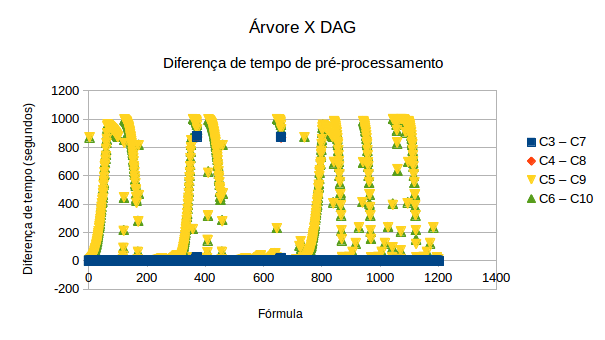
\includegraphics[scale=.5]{arvore_x_dag_time}
	\end{center}
	
	\vspace{-.6cm}
	\pause Claro, DAG é uma estrutura mais compacta!
\end{frame}

\begin{frame}{Resultados e análise}{Comparações entre árvores e DAGs}
	Combinações $3,4,5,6$: árvore\\
	Combinações $7,8,9,10$: DAG
	
	\vspace{-.4cm}
	\pause
	\begin{center}
		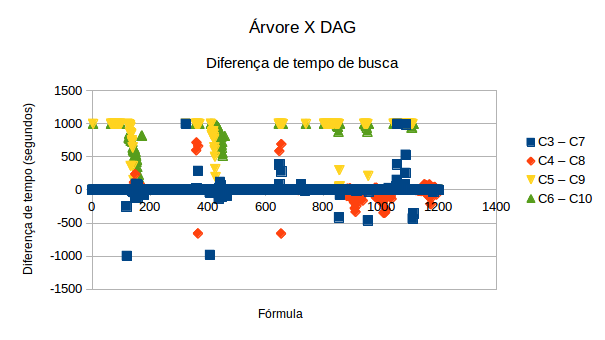
\includegraphics[scale=.5]{arvore_x_dag_ptime}
	\end{center}
	
	\vspace{-.6cm}
	\pause Primeiro indício! \pause Converter para DAG é essencial.
\end{frame}

\begin{frame}{Resultados e análise}{Comparações entre os algoritmos de renomeamento}
	Combinações $7,8$: Boy de la Tour, sem e com simplificação\\
	Combinações $9,10$: Algoritmo proposto, sem e com simplificação
	
	\pause \begin{center}Comparando número de cláusulas.\end{center}
	\begin{itemize}
		\pause\item A transformação terminou em C7 e C9 para 73\% das fórmulas.
		\pause\item Em 3\%, a transformação terminou em C7 e C9 e C7 produziu menos cláusulas, com $\max \{|C7-C9| \} = 3$.
		\pause\item Em 8\%, a transformação terminou em C7 e C9 e C9 produziu menos cláusulas, com $\max \{|C7-C9| \} = 1.572.786$, onde C9 produziu 78 cláusulas.
	\end{itemize}
\end{frame}

\begin{frame}{Resultados e análise}{Comparações entre os algoritmos de renomeamento}
	Combinações $7,8$: Boy de la Tour, sem e com simplificação\\
	Combinações $9,10$: Algoritmo proposto, sem e com simplificação
	
	\vspace{-.4cm}
	\pause
	\begin{center}
		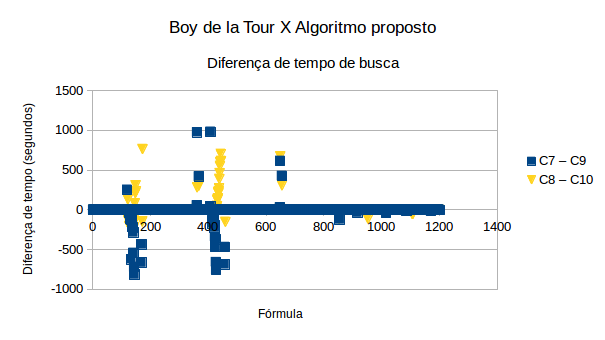
\includegraphics[scale=.5]{boy_x_knapsack_ptime}
	\end{center}
	
	\vspace{-.6cm}
	\pause Cada algoritmo leva vantagem em famílias de fórmulas específicas.
\end{frame}

\begin{frame}{Resultados e análise}{Tempo de busca em função do número de cláusulas}
	\begin{center}
		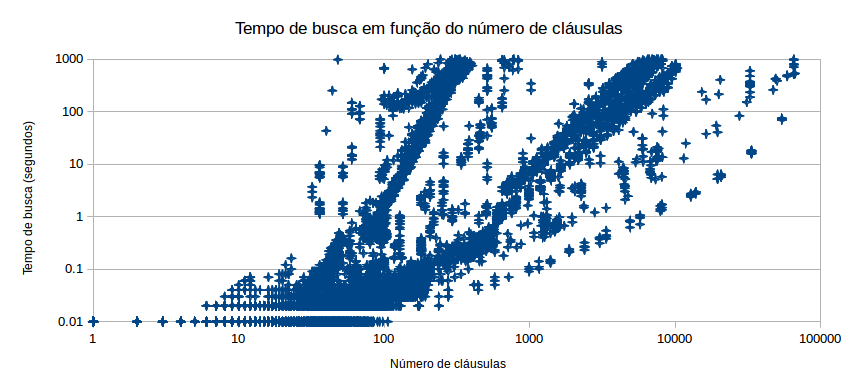
\includegraphics[scale=.45]{ptime}
	\end{center}
\end{frame}

\begin{frame}{Resultados e análise}{Tempo de busca em função do número de cláusulas}
	\begin{center}
		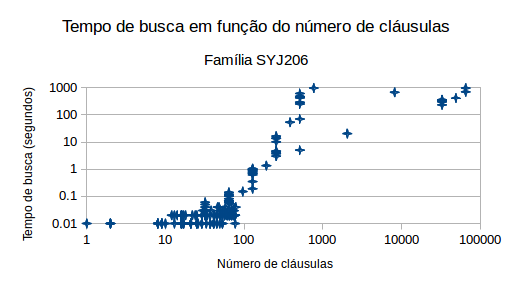
\includegraphics[scale=.6]{ptime_SYJ}
	\end{center}
	
	\pause Então, sim!
\end{frame}


\label{cap_conclusoes}

Conclusões

\section{Referências}

\begin{frame}[allowframebreaks]
  \frametitle{Referências}
  \bibliographystyle{ieeetr}
  \bibliography{referencias}
\end{frame}

\end{document}
